\documentclass[border=1cm]{standalone}

\usepackage{tikz}
\usepackage{tikzducks}

\begin{document}

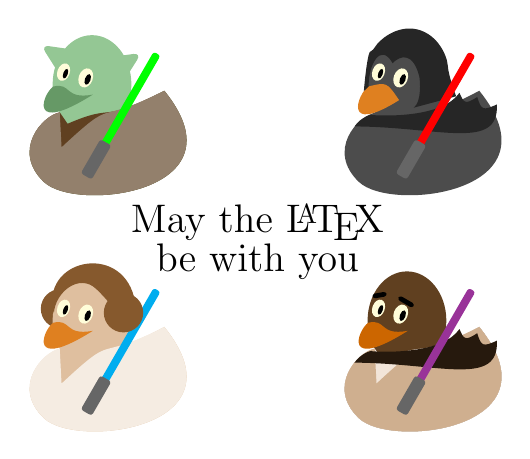
\begin{tikzpicture}
\colorlet{skin}{white!45!gray!80!green}

\duck[
    lightsaber,
    body=skin,
    bill=gray!80!green,
    tshirt=brown!50!black,
    jacket=brown!30!gray
  ];
  \fill[skin,rounded corners=3] (0.44,1.70) -- (0.25,2) -- (0.6,1.95);
  \fill[skin,rounded corners=3] (1.34,1.60) -- (1.53,1.9) -- (1.16,1.85);

\duck[
    grumpy,
    lightsaber=red,
    cape=black!85!white,
    body=black!70!white,
    darthvader=black!85!white,
    xshift=4cm,
  ];

\fill[brown!70!black] (0.5,1.65-3) circle (0.25);
  \duck[
    jacket=white!85!brown,
    body=brown!50!white,
    shorthair=brown!70!black,
    lightsaber=cyan,
    yshift=-3cm,
  ]
  \fill[brown!70!black] (1.3,1.6-3) circle (0.25);

      \duck[
        body=brown!50!black,           % Kolor skóry
        bill=orange!80!black,    % Dziób (lekko przyciemniony, by pasował)
        eyebrow=black,           % Groźne/poważne brwi
        jacket=orange!25!lightgray,          % Wewnętrzna tunika (kamizelka)
        tshirt=brown!20!white,
        cape=brown!20!black,          % Zewnętrzna szata (peleryna)
        lightsaber=violet!80!white,
        xshift=4cm, yshift=-3cm
    ];
    
\node[align=center] at (3,-0.5) {\Large May the \LaTeX \\\Large be with you};

\end{tikzpicture}

\end{document}